\documentclass[a4paper,10pt]{article}
\usepackage[utf8]{inputenc}
\usepackage{url}
\usepackage{amsmath}
\usepackage{graphicx}

%opening
\title{COMP417: Assignment 3\\Due Friday, March 24  at 6pm}
\author{}

\begin{document}

\maketitle


\section{Occupancy grid mapping (5pts)}
In this exercise you are going to implement parts of the occupancy grid mapping system discussed in class. In particular, you are going to map an environment 
based on known odometry estimates and known 2D laser scans. Do \path{git} $\;$ \path{pull} under your comp417 repository to get the starter code. The functionality 
that you need to implement is marked using to-do comments in the file \path{estimation_assignment/python/occupancy_grid_mapper.py}. To run your code, 
\path{cd} $\;$ \path{path/to/comp417/estimation_assignment/} and execute the following commands on three different terminals: 
\newline

  \path{rosbag} $\;$ \path{play} $\;$ \path{laser_and_odometry.bag}
  
  \path{roslaunch} $\;$ \path{estimation_assignment} $\;$ \path{occupancy_grid_mapping.launch} $\;$ \path{odometry_orientation_noise_std_dev:=2.5} $\;$ \path{odometry_position_noise_std_dev:=0.1}
  
  \path{rosrun} $\;$ \path{rviz} $\;$ \path{rviz} 
\newline
\newline
\noindent When rviz initializes, go to \path{File} $>$ \path{Open Config} and then load the configuration file in \path{estimation_assignment/resources/comp417.rviz}
which is going to start the visualization of laser scan messages, frames of reference, and debugging visualizations. Save this configuration file as the default
in your \path{/home/username/.rviz/default.rviz}, so you won't have to do this every time you restart rviz. In the \path{roslaunch} command given above, the standard deviation of 
the odometry orientation noise is given in degrees. In this example the true yaw of the robot is corrupted by random noise from $\mathcal{N}(0, 2.5^2)$. Similarly, the true position 
is corrupted by random noise from $\mathcal{N}(0, 0.1^2)$, which is expressed in meters. \path{laser_and_odometry.bag} is a recording of laser scans and odometry data in the environment 
you used in Assignment 1. The expected result for perfect odometry looks similar to Figure \ref{fig:gmapping}. 
\newline
\begin{figure}[h]
  \begin{center}
    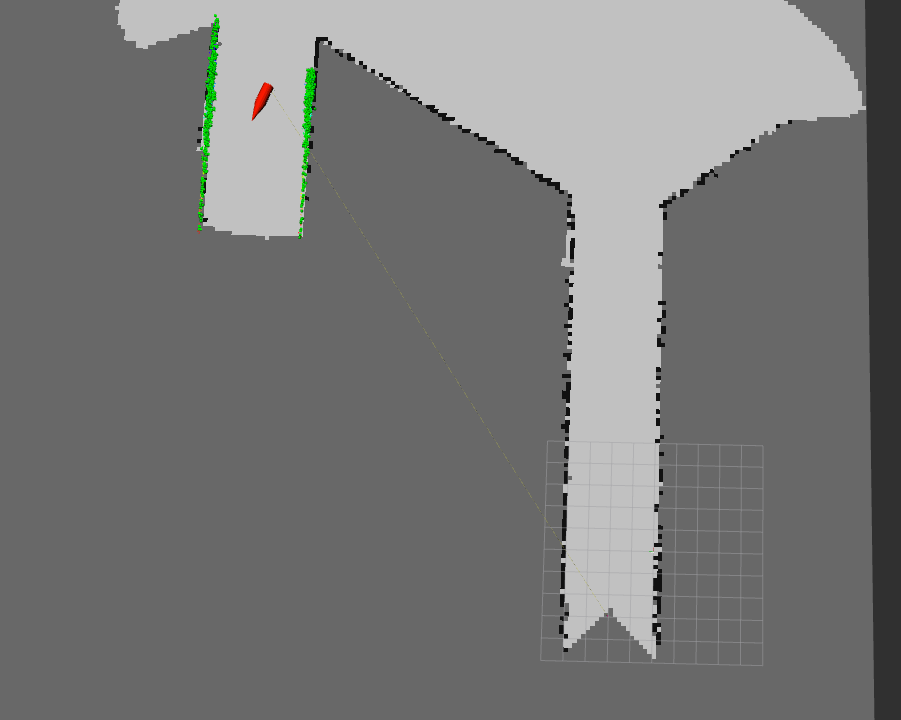
\includegraphics[width=0.5\textwidth]{gmapping}
  \end{center} 
  \caption{Part of the robot's mapping task during the (0,0) noise trajectory.}
  \label{fig:gmapping}
\end{figure}
\newline
\newline
\noindent What you need to submit: 5 images of maps produced by your mapper, with noise parameters (0, 0), (2.5, 0), (5, 0), (2.5, 0.1), (5, 0.1) respectively. 
Your images should be named \path{map_[0|1|2|3|4]_firstname_lastname.png}. Also, submit a video recording of the rviz visualization for the odometry noise combination (0,0),
demonstrating your map being built from beginning to end. Your video should be named \path{map_0_firstname_lastname.mp4/avi/ogg}. 

\section{Least squares localization (5pts)}
In this exercise you are going to solve the localization problem in a map of known landmarks. In particular, assume your robot
has 2D state $\textbf{x}_t=[p_x(t) \; p_y(t)]^T$ and an omnidirectional motion model $\textbf{x}_{t+1}=\textbf{x}_t + \textbf{u}_t\delta t + \textbf{w}_t$, where $\textbf{w}_t \sim \mathcal{N}(0, \sigma_w^2\textbf{I})$
The robot is moving through an environment that has L static landmarks $\textbf{l}_1, ..., \textbf{l}_L$ whose positions are known.
Occasionally the robot makes the following set of measurements: $z_t^{(i)}=||\textbf{x}_t-\textbf{l}_i||+n_t$ where $n_t \sim \mathcal{N}(0, \sigma_n^2)$, for some of the available landmarks.
Your goal is to estimate the sequence of states $\textbf{x}_{1:T}$ by minimizing a least squares cost function. 
\newline
\newline
\noindent You can find starter code in \path{estimation_assignment/python/localization.py}. It provides the set of measurements made at each timesteps. Your task is to implement the cost 
function using \path{numpy} and the nonlinear least squares solver in \path{scipy.optimize.least_squares}. There are to-do comments in the code that explain in detail what you need to implement. 
After you are done with your implementation, the expected outcome is the following figure:
\begin{figure}[h]
  \begin{center}
    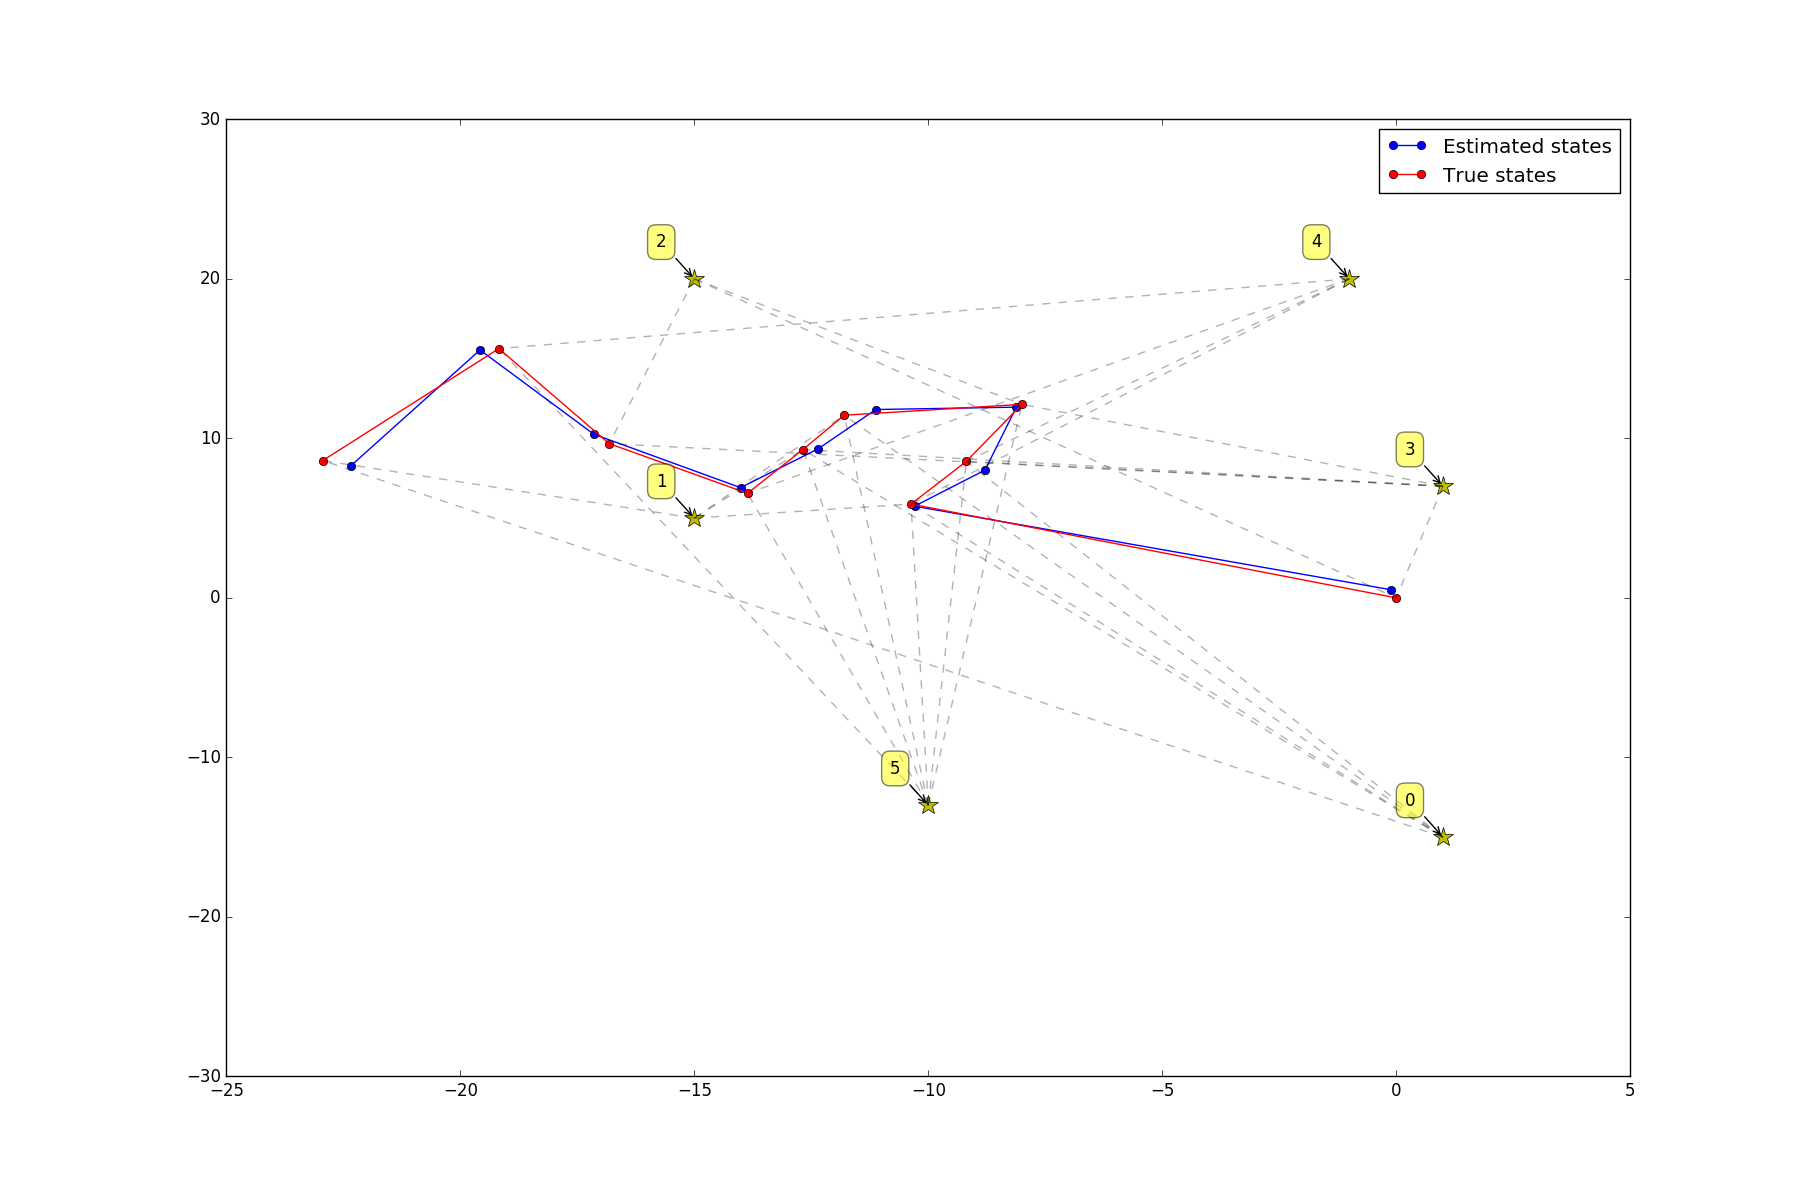
\includegraphics[width=\textwidth]{localization}
  \end{center} 
  \caption{The robot starts at (0,0) and moves throughout the world, making measurements of static, known landmarks.}
\end{figure}

\noindent What you need to submit: your code in the file \path{estimation_assignment/python/localization.py}.
\newline
\newline
P.S.: You can think of cell phone localization based on static cell towers as a particular application of this problem.  

\subsection{Bonus (1pt)}
Try to convert this localization problem into range and bearing GraphSLAM. The dynamics of the robot should be those of the Dubins car. 
The measurement model should consist of the range and the bearing of a landmark with respect to the robot's body frame. If you do
this bonus question save your work in a file called \path{estimation_assignment/python/graphslam.py} 

\subsection{Bonus (1pt)}
Try to implement the localization problem given above in one of the following three frameworks, which specialize in solving least squares
problems in robotics: \path{GTSAM}\footnote{\url{https://collab.cc.gatech.edu/borg/gtsam}}, \path{g2o}\footnote{\url{https://github.com/RainerKuemmerle/g2o}}, \path{Ceres}\footnote{\url{http://ceres-solver.org/}}. 
Depending on your choice of framework, and whether you use Python bindings or not, this might involve writing a C++ version of the starter code provided above.


\section{Extended Kalman Filter (2.5pts)}
Assume you have a robot that follows Dubins car dynamics on the plane. Its state is $\textbf{x}_t=[p_x(t) \; p_y(t) \; \theta(t)]$. Also assume that you have
three landmarks $\textbf{l}_i=[l_x^{(i)} \; l_y^{(i)}]$ in the world. At each point in time the robot observes all three landmarks, with some sensor noise.
The measurement model consists of the Euclidean distances from the robot's current state to each of the three landmarks, plus noise. Formulate an EKF estimator for this problem.
Specifically, formally define the dynamics model, the observation model, their Jacobians, and the covariances of their noise processes. There is no implementation
required for this question, but if you want to do it, you can find starter code at \path{path/to/comp417/filtering_examples/python}. 

\section{How to submit}
Submit all your work in a file called \path{estimation_assignment.zip} that contains your extensions to the provided starter code, as well as the five images, the video, and the pdf file. 
Submissions will be done on myCourses. 

\section{A note on indentation}
Please make sure your editor uses spaces instead of tab characters, otherwise your TAs will have a hard time reading your code on their editors, which might be different from yours.
\end{document}
